

\documentclass[12pt]{article}
\usepackage{amsfonts, epsfig}
\usepackage{amsmath}
\usepackage{graphicx}
\usepackage{pstricks}
\usepackage{listings}

\usepackage{tikz}
\usetikzlibrary{positioning}
\usetikzlibrary{arrows,automata}
\usetikzlibrary{decorations.markings}
\usetikzlibrary{calc}



%\usepackage{tikzscale}
%\usepackage{pgfplots}

%\pgfplotsset{compat=1.8}

\usepackage{fancyhdr}
\pagestyle{fancy}
\lfoot{\texttt{coms30127.github.io}}
\lhead{Computation Neuroscience - 06.2\_synaptic\_plasticity - Conor}
\rhead{\thepage}
\cfoot{}


\usepackage{ifthen}
\newboolean{nopics}
\setboolean{nopics}{false}

\begin{document}

\section*{Synaptic plasticity}

Synaptic plasticity usually refers to the long-term changes in synapse
strength, an long term increase in synaptic strength is called
\textsl{long term potentiation} of LTP, a decrease is called
\textsl{long term depression} or LTD. It is believed that synapses
respond to their pre- and post-synaptic activity, so that the changes
depend on the behavior of the pre- and post-synaptic neurons. It is
not known in detail what rules govern this plasticity, it seems
different neurons have different plasticity rules. 

The closest thing to an overall rule was formulated by Hebb in 1949
when he said \cite{Hebb1949a}:
\begin{quote}
Let us assume that the persistence or repetition of a reverberatory
activity (or \lq{}trace\rq{}) tends to induce lasting cellular changes that
add to its stability. [$\ldots$] When an axon of cell A is near enough to excite
a cell B and repeatedly or persistently takes part in firing it, some
growth process or metabolic change takes place in one or both cells
such that A's efficiency, as one of the cells firing B, is increased.
\end{quote}
In other words, if one neurons tends to cause another to fire, the
synapse from the first to the second will get stronger. In artificial
neural networks the nodes, modelling neurons, often lack spiking
dynamics and so have a continuous state or rate variable; since
\textsl{Hebbian plasticity} often plays a role in artificial neural
networks it is often applied to a rule that strengthens synapses
between neurons that are active at the same time, that is, the
explicit causal structure is ignored in favor of
\begin{quote}
Neurons that fire together wire together.
\end{quote}
This leads to a plasticity rule 
\begin{equation}
\delta w_{ij}=\eta x_i x_j
\end{equation}
where $w_{ij}$ is the strength of the synapse from neuron $i$ to
neuron $j$, $x_i$ and $x_j$ are the states of the two neurons and
$\eta$ is a learning rate. Another version is
\begin{equation}
\delta w_{ij}=\eta (x_i-\theta)(x_j-\theta)
\end{equation}
where $\theta$ is a threshold, this allows negative changes, when
$x_i>\theta$ and $x_j<\theta$, or visa versa.

\subsection*{Spike-timing dependent plasticity}

The late nineties saw a revival of interest in causal, spike-timing
dependent plasticity (STDP). A series of papers pointed to experimental
evidence for timing effects in plasticity
\cite{MarkramSakmann1995a,MarkramEtAl1997a,BellEtAl1997a,MageeJohnston1997a,DebanneGahwilerThompson1998a}
including a definitive demonstration of a STDP changes \textsl{in vitro} in \cite{MarkramEtAl1997a}, the
observation of asymmetric STDP \textsl{in vivo} in developing Xenopus
in \cite{ZhangTaoHoltHarrisPoo1998a} and a clear graph of the time
dependence of plastic changes \textsl{in vitro} in \cite{BiPoo1998a}.

The famous graph of STDP is shown in
Fig.~\ref{fig:BiPoo}. This shows measurements of plastic changes made
in an \textsl{in vitro} preparation. Electrodes are inserted into two
synaptically connected cells and currents are used to cause both to
spike periodically with a gap of $\delta t$ between the pre- and
post-synaptic spikes. This causes the synaptic strength to change, if
the pre-synaptic spike precedes the post-synaptic spike the synapse
gets stronger with the degree of strengthening depending on the size
of $|\delta t|$, the bigger the gap the smaller the effect with a
roughly exponential profile. The opposite is observed if the
pre-synaptic spike arrives after the post-synaptic spike has left, in
this case the synapse gets weaker, again the size of the effect falls
like an exponential as $|\delta t|$ gets bigger.


\begin{figure}
  \ifthenelse{\boolean{nopics}}
             {\textsl{The horizontal axis runs from -200 ms to  50 ms, the vertical axis from 0 to 250 corresponding to the relativing timing of the pre- and post-synaptic spike. Negative corresponds to pre- after post-, the acausal case. The vertical axis is marked `Normalized EPSP slope (\%)'. There are two exponential curves, one on the negative side, stopping at the 0 ms point along the horizontal axis, the one on the positive side is likewise only on the side corresponding to positive values for the horizontal axis. The curve on the negative side a curve starts near zero and approach a value of about -50\%, in otherwords it is negative, the curve on the positive side starts at around 175\% at the 0 ms point and falls towards zero by the time it reaches 50 ms, in otherwords it has a much smaller timescale. Around each curve there are lots of points, indicating that the curves match some noisy data. }
             }            
{  \begin{center}
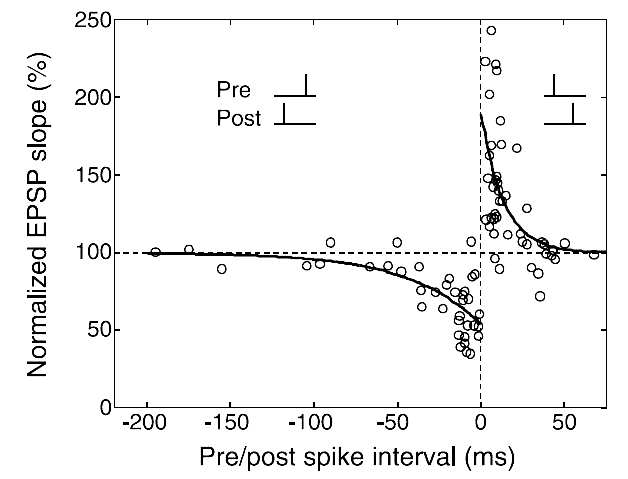
\includegraphics[width=12cm]{DanPoo2004.jpg}
\end{center}}
\caption{Spike timing dependent plasticity. This shows the change in
  synapse strength as a function of the timing gap between the pre-
  and post-synaptic spike. \label{fig:BiPoo}}
\end{figure}

There are lots of caveats to be added to this, it is quite an
artificial situation, in vitro with periodic spiking; since the
changes are only tracked over a show period it isn't clear whether the
changes are additive
\begin{equation}
w\rightarrow w+\delta w
\end{equation}
or multiplicative
\begin{equation}
w\rightarrow \lambda_w w
\end{equation}
However, it does give a striking picture of how STDP might work. 


\begin{figure}
  \ifthenelse{\boolean{nopics}}
             {\textsl{Nodes in a line are connected to single nodes below them, the upper row is labelled `retinal layer' and although only six nodes are shown it is indicated that there are actually 1000 grouped in two groups of 500. The lower neuron is labelled `V1'.}}
             {
\begin{center}
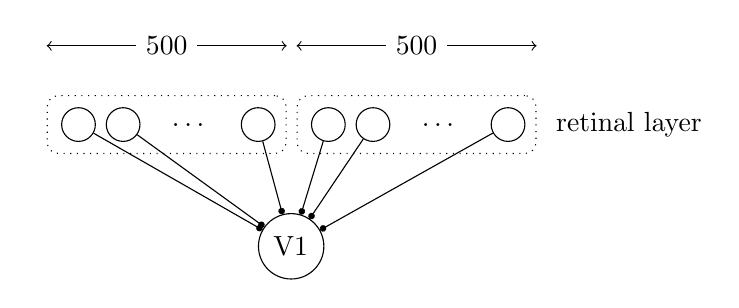
\begin{tikzpicture}
\node[rectangle,rounded corners,text width=2.8cm,text height=0.5cm,draw=black,dotted,align=left](a){};
\node[rectangle,rounded corners,text width=2.8cm,text height=0.5cm,draw=black,dotted,align=left, right = 0.125cm of a](b){};
\node[align=left, right = 0.125cm of b](text){retinal layer};
\node[left = 0cm of a](al){};
\node[right = 0cm of a](ar){};
\node[above of = al](aal){};
\node[above of = ar](aar){};
\node[above of = a](atext){500};
\path (atext) edge[->] (aal);
\path (atext) edge[->] (aar);
\node[left = 0cm of b](bl){};
\node[right = 0cm of b](br){};
\node[above of = bl](abl){};
\node[above of = br](abr){};
\node[above of = b](btext){500};
\path (btext) edge[->] (abl);
\path (btext) edge[->] (abr);

\node[right = -0.0675cm of a](ab){};

\node[circle,text width=0.125cm,draw=black,align=center,left = -0.625cm of a](a1){};
\node[circle,text width=0.125cm,draw=black,align=center,right = 0.125cm of a1](a2){};
\node[text width=0.125cm,align=center,right = 0.275cm of a2](adots){$\ldots$};
\node[circle,text width=0.125cm,draw=black,align=center,right = 0.625cm of adots](a3){};
\node[circle,text width=0.125cm,draw=black,align=center,left = -0.625cm of b](b1){};
\node[circle,text width=0.125cm,draw=black,align=center,right = 0.125cm of b1](b2){};
\node[text width=0.125cm,align=center,right = 0.275cm of b2](bdots){$\ldots$};
\node[circle,text width=0.125cm,draw=black,align=center,right = 0.625cm of bdots](b3){};

\node[circle,text width=0.45cm,draw=black,align = left,below = 1cm of ab](pc){V1};


\draw[
    decoration={markings,mark=at position 1 with {\arrow[scale = 0.5]{*}}},
    postaction={decorate}
    ]
    (a1) -- (pc);

\draw[
    decoration={markings,mark=at position 1 with {\arrow[scale = 0.5]{*}}},
    postaction={decorate}
    ]
    (a2) -- (pc);

\draw[
    decoration={markings,mark=at position 1 with {\arrow[scale = 0.5]{*}}},
    postaction={decorate}
    ]
    (a3) -- (pc);

\draw[
    decoration={markings,mark=at position 1 with {\arrow[scale = 0.5]{*}}},
    postaction={decorate}
    ]
    (b1) -- (pc);

\draw[
    decoration={markings,mark=at position 1 with {\arrow[scale = 0.5]{*}}},
    postaction={decorate}
    ]
    (b2) -- (pc);

\draw[
    decoration={markings,mark=at position 1 with {\arrow[scale = 0.5]{*}}},
    postaction={decorate}
    ]
    (b3) -- (pc);


\end{tikzpicture}
\end{center}
}
\caption{The STDP of Song and Abbott. 1000 input neurons, refered to
  as retinal neurons, feed forward to a single V1 neuron. The retinal
  neurons are divided into two groups: the first 500 and the second
  500, the two groups provide noisy output, these give the input to
  the V1 neuron. The inputs from neurons in the same group are
  correllated, meaning they are more likely to be similar to each other in their activity than neurons from different groups.\label{fig:sa_stdp}}
\end{figure}

In fact, an example of how STDP might support unsupervized learning
was given in \cite{SongEtAl2000a,SongAbbott2001a}. A toy model is
introduced with multiple neuron inputs feeding forward to a single
integrate-and-fire neuron. The inputs are divided into two groups and
given a correlation structure so that inputs in the same group are
more likely to spike at roughly the same time. This is sketched in
Fig.~\ref{fig:sa_stdp}. The synapses are then adjusted according to a
simple STDP rule. It is seen that one of the two groups \lq{}wins
out\rq{}, its synapses get stronger while the synapses corresponding
to the other group gets weaker. Basically if one group, by chance, is
slightly more likely to cause the post-synaptic neuron to spike than
the other, then the post-synaptic spikes are more likely to occur
after the pre-synaptic spikes for that group, so the synapses will get
stronger, increasing the effect.


\begin{figure}
  \ifthenelse{\boolean{nopics}}
             {\textsl{Before and after pictures. In each case there are 1000 crosses evenly spaced horizontally, corresponding to 1000 synapse strengths. The vertical axis runs from zero to one. In the before picture the crosses are randomly distributed between zero and one, in the after picture the first 500 are mostly near zero and the second 500 mostly near one.
                 }}
{
  % GNUPLOT: LaTeX picture with Postscript
\begingroup
  \makeatletter
  \providecommand\color[2][]{%
    \GenericError{(gnuplot) \space\space\space\@spaces}{%
      Package color not loaded in conjunction with
      terminal option `colourtext'%
    }{See the gnuplot documentation for explanation.%
    }{Either use 'blacktext' in gnuplot or load the package
      color.sty in LaTeX.}%
    \renewcommand\color[2][]{}%
  }%
  \providecommand\includegraphics[2][]{%
    \GenericError{(gnuplot) \space\space\space\@spaces}{%
      Package graphicx or graphics not loaded%
    }{See the gnuplot documentation for explanation.%
    }{The gnuplot epslatex terminal needs graphicx.sty or graphics.sty.}%
    \renewcommand\includegraphics[2][]{}%
  }%
  \providecommand\rotatebox[2]{#2}%
  \@ifundefined{ifGPcolor}{%
    \newif\ifGPcolor
    \GPcolorfalse
  }{}%
  \@ifundefined{ifGPblacktext}{%
    \newif\ifGPblacktext
    \GPblacktexttrue
  }{}%
  % define a \g@addto@macro without @ in the name:
  \let\gplgaddtomacro\g@addto@macro
  % define empty templates for all commands taking text:
  \gdef\gplbacktext{}%
  \gdef\gplfronttext{}%
  \makeatother
  \ifGPblacktext
    % no textcolor at all
    \def\colorrgb#1{}%
    \def\colorgray#1{}%
  \else
    % gray or color?
    \ifGPcolor
      \def\colorrgb#1{\color[rgb]{#1}}%
      \def\colorgray#1{\color[gray]{#1}}%
      \expandafter\def\csname LTw\endcsname{\color{white}}%
      \expandafter\def\csname LTb\endcsname{\color{black}}%
      \expandafter\def\csname LTa\endcsname{\color{black}}%
      \expandafter\def\csname LT0\endcsname{\color[rgb]{1,0,0}}%
      \expandafter\def\csname LT1\endcsname{\color[rgb]{0,1,0}}%
      \expandafter\def\csname LT2\endcsname{\color[rgb]{0,0,1}}%
      \expandafter\def\csname LT3\endcsname{\color[rgb]{1,0,1}}%
      \expandafter\def\csname LT4\endcsname{\color[rgb]{0,1,1}}%
      \expandafter\def\csname LT5\endcsname{\color[rgb]{1,1,0}}%
      \expandafter\def\csname LT6\endcsname{\color[rgb]{0,0,0}}%
      \expandafter\def\csname LT7\endcsname{\color[rgb]{1,0.3,0}}%
      \expandafter\def\csname LT8\endcsname{\color[rgb]{0.5,0.5,0.5}}%
    \else
      % gray
      \def\colorrgb#1{\color{black}}%
      \def\colorgray#1{\color[gray]{#1}}%
      \expandafter\def\csname LTw\endcsname{\color{white}}%
      \expandafter\def\csname LTb\endcsname{\color{black}}%
      \expandafter\def\csname LTa\endcsname{\color{black}}%
      \expandafter\def\csname LT0\endcsname{\color{black}}%
      \expandafter\def\csname LT1\endcsname{\color{black}}%
      \expandafter\def\csname LT2\endcsname{\color{black}}%
      \expandafter\def\csname LT3\endcsname{\color{black}}%
      \expandafter\def\csname LT4\endcsname{\color{black}}%
      \expandafter\def\csname LT5\endcsname{\color{black}}%
      \expandafter\def\csname LT6\endcsname{\color{black}}%
      \expandafter\def\csname LT7\endcsname{\color{black}}%
      \expandafter\def\csname LT8\endcsname{\color{black}}%
    \fi
  \fi
  \setlength{\unitlength}{0.0500bp}%
  \begin{picture}(4320.00,3724.00)(0,-200)%
    \gplgaddtomacro\gplbacktext{%
      \csname LTb\endcsname%
      \put(900,3400){\makebox(0,0){\strut{}\textbf{before}}}%
   \put(946,442){\makebox(0,0)[r]{\strut{} 0}}%
      \put(946,905){\makebox(0,0)[r]{\strut{} 0.2}}%
      \put(946,1368){\makebox(0,0)[r]{\strut{} 0.4}}%
      \put(946,1831){\makebox(0,0)[r]{\strut{} 0.6}}%
      \put(946,2294){\makebox(0,0)[r]{\strut{} 0.8}}%
      \put(946,2757){\makebox(0,0)[r]{\strut{} 1}}%
      \put(1081,220){\makebox(0,0){\strut{} 0}}%
      \put(2501,220){\makebox(0,0){\strut{} 500}}%
      \put(3920,220){\makebox(0,0){\strut{} 1000}}%
%      \put(176,1599){\rotatebox{90}{\makebox(0,0){\strut{}$w_i / w^{max}$}}}%
      \put(2501,-200){\makebox(0,0){\strut{}synapse index $i$}}%
      \put(5400,3400){\makebox(0,0){\strut{}\textbf{after}}}%
      \put(5446,442){\makebox(0,0)[r]{\strut{} 0}}%
      \put(5446,905){\makebox(0,0)[r]{\strut{} 0.2}}%
      \put(5446,1368){\makebox(0,0)[r]{\strut{} 0.4}}%
      \put(5446,1831){\makebox(0,0)[r]{\strut{} 0.6}}%
      \put(5446,2294){\makebox(0,0)[r]{\strut{} 0.8}}%
      \put(5446,2757){\makebox(0,0)[r]{\strut{} 1}}%
      \put(5581,220){\makebox(0,0){\strut{} 0}}%
      \put(7001,220){\makebox(0,0){\strut{} 500}}%
      \put(8420,220){\makebox(0,0){\strut{} 1000}}%
      \put(7001,-200){\makebox(0,0){\strut{}synapse index $i$}}%
%      \put(4676,1599){\rotatebox{90}{\makebox(0,0){\strut{}$w_i / w^{max}$}}}%
    }%
    \gplgaddtomacro\gplfronttext{%
    }%
    \gplbacktext
    \put(0,0){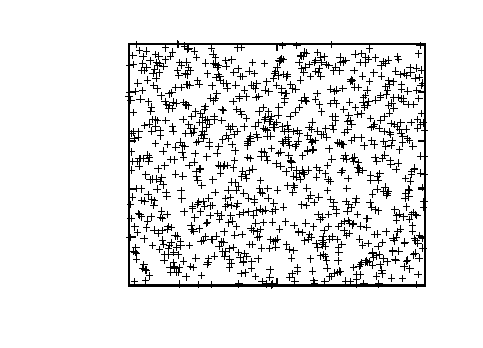
\includegraphics{synapses_before}}%
\put(4500,0){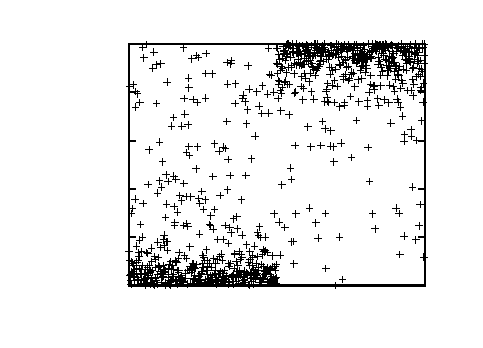
\includegraphics{synapses_after}}%
    \gplfronttext
  \end{picture}%
\endgroup
}
\caption{Synapse strengths before and after in Song and Abbotts simple model. At first they are all random, after the STDP has had an effect the synapses from one of the two groups have approached their maximum value, the others are near zero. \label{fig:before_after}}
\end{figure}

\begin{thebibliography}{10}

\bibitem{AbbottEtAl1997a}
Abbott LF, Varela JA, Sen K and Nelson SB. (1997) Synaptic depression and cortical gain control. 
\newblock Science, 275: 221--224.

\bibitem{Hebb1949a}
Hebb DO. (1949) The Organization of Behavior. 
\newblock New York: Wiley \& Sons.

\bibitem{MarkramSakmann1995a}
Markram H, Sakmann B (1995) Action potentials propogating back into dendrites triggers changes in efficacy of single-axon synapses between layer V pyramidal cells. 
\newblock Society of Neuroscience Abstract 21.

\bibitem{MarkramEtAl1997a}
Markram H, {L\"{u}bke} J, Frotscher M, Sakmann B (1997) Regulation of synaptic
  efficacy by coincidence of postsynaptic aps and epsps.
\newblock Science 275: 213-215.

\bibitem{BellEtAl1997a} 
Bell CC, Han VZ, Sugawara Y, Grant K (1997) Synaptic plasticity in a
cerebellum-like structure depends on temporal order.
\newblock Nature 387: 278--281.

\bibitem{MageeJohnston1997a}
Magee JC, Johnston D (1997) A synaptically controlled, associative signal for
  Hebbian plasticity in hippocampal neurons.
\newblock Science 275: 209--213.

\bibitem{DebanneGahwilerThompson1998a}
Debanne D, {G\"{a}hwiler} BH, Thompson SM (1998) Long-term synaptic plasticity
  between pairs of individual ca3 pyramidal cells in rat hippocampal slice
  cultures.
\newblock Journal of Physiology 507: 237--247.

\bibitem{ZhangTaoHoltHarrisPoo1998a}
Zhang LI, Tao HW, Holt CE, Harris WA, Poo MM (1998). A critical window for cooperation and competition among developing retinotectal synapses. 
\newblock Nature 395: 37--44.

\bibitem{BiPoo1998a}
Bi G, Poo M (1998) Synaptic modifications in cultured hippocampal neurons:
  Dependence on spike timing, synaptic strength, and postsynaptic cell type.
\newblock Journal of Neuroscience 18: 10464--10472.

\bibitem{SongEtAl2000a}
Song S, Miller K, Abbott L (2000) Competitive hebbian learning through
  spike-timing-dependent synaptic plasticity.
\newblock Nature Neuroscience 3: 919--926.

\bibitem{SongAbbott2001a}
Song S, Abbott L (2001) Cortical development and remapping through spike
  timing-dependent plasticity.
\newblock Neuron 32: 339-350.


\end{thebibliography}

\end{document}
